\chapter{Pages bonus !}

	\section{Formules mathématiques}
	
		Pour effectuer des calculs de probabilités, il est possible d'utiliser la formule de Bayes:
		\begin{equation}
			p(B_i/A)=\frac{p(A/B_i)p(B_i)}{\sum_{i=1}^{n}p(A|B_i)p(B_i)}
		\end{equation}
		
		Pour un lancé de \og pile ou face\fg{}, l'univers $ \Omega $ de cette expérience sera le suivant:
		\[\Omega={pp, pf, fp, ff}\]
		
		La fonction de répartition de cette expérience sera donc:
		\[ 
			F_X(x)
			\begin{cases}
				0 & \text{si } x \in ]-\infty,0[ \\
				\frac{1}{4} & \text{si } x \in [0,1[ \\
				\frac{3}{4} & \text{si } x \in [1,2[ \\
				1 & \text{si } x \in [2,+\infty[ \\
			\end{cases}
		\]
	
	\section{Graphiques}
	
		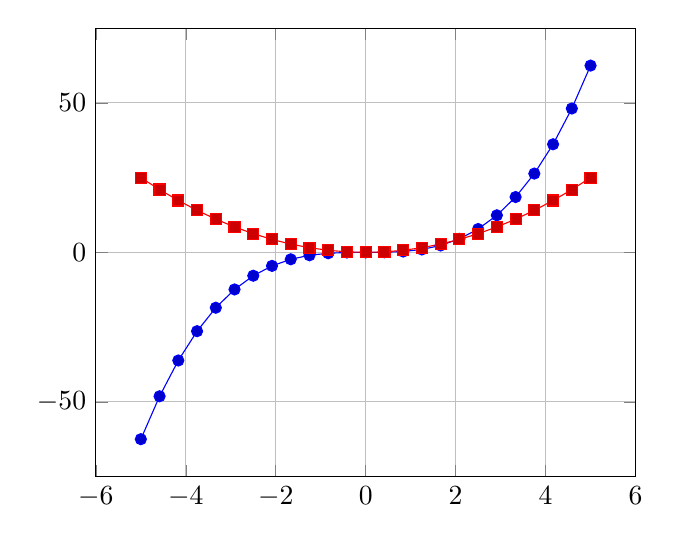
\begin{tikzpicture}
			\begin{axis}[grid=major, domain=-5:5]
				\addplot {(1/2)*x^3};
				\addplot {x^2};
			\end{axis}
		\end{tikzpicture}
		
		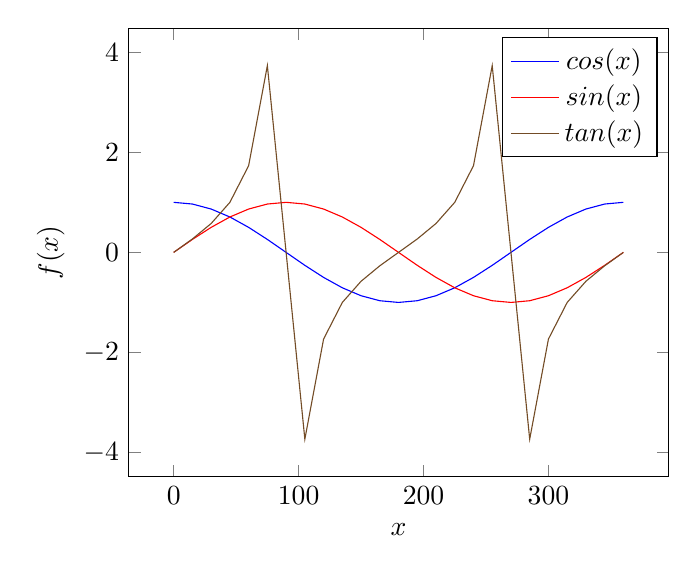
\begin{tikzpicture}
			\begin{axis}[domain=0:360, no markers, xlabel=$x$, ylabel=$f(x)$]
				\addplot {cos(x)};
				\addplot {sin(x)};
				\addplot {tan(x)};
				\legend{$cos(x)$, $sin(x)$,$tan(x)$}
			\end{axis}
		\end{tikzpicture}
	
	\section{Unités}
	
		La vitesse de la lumière est de \SI{3e8}{\m\per\second}.
		
		Nous sommes le jeudi 3 mai 2018 et la température est de \SI{13}{\celsius}.
		
	\section{Tableau de nombres}
	
		\begin{tabular}{|S|}
			\hline
			{Températures de la journée} \\
			\hline
			9.6 \\
			12 \\
			13.24 \\
			12.7835 \\
			\hline
		\end{tabular}